\section{Related Work}
\label{sec:related_work}

\begin{figure}[t]
    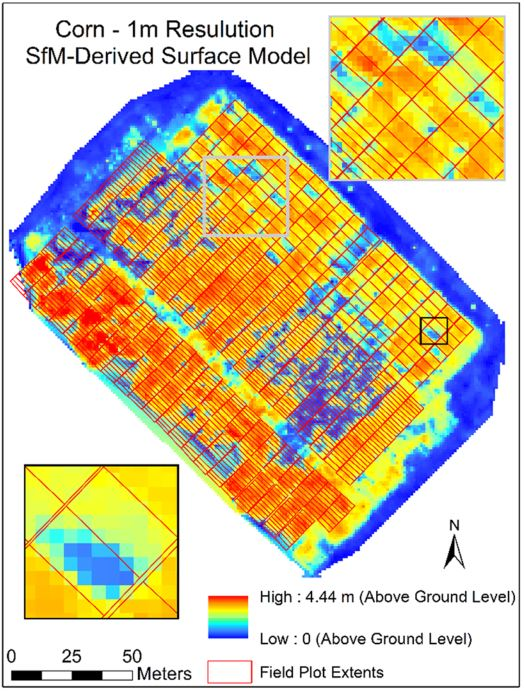
\includegraphics[width=\linewidth]{../images/DSM} 
    \caption{Digital surface models (DSMs). From \cite{UAV_HTPAR_2016}.}
    \label{fig:DSM}
\end{figure}

This work builds on the research "Unmanned Aerial Vehicles for High-Throughput Phenotyping and Agronomic Research" \cite{UAV_HTPAR_2016}.
The authors provided four case studies involving multiple crops in breeding and agronomic applications developed by five teams: Administration, Flight Operations, Sensors, Data Management and Field Research. As the first project of its kind, it provided valuable lessons learned about critical informations of sensors, air vehicles and configuration parameters for both.
Images from a large field of maize for a total of 1064 plots were collected using a UAV equipped with a high-resolution camera on July 22, 2015.
A digital surface model (DSM) [\ref{fig:DSM}] was calculated from the image data and used to estimate height. The height estimates were compared to ground truth measurements taken approximately three weeks earlier.
The approach used in this study resulted in a correlation of ($r^2 = 0.35$; $p<0.0001$) for the first case study, where only 705 plots were analyzed as a group because a significant number of plots sustained extensive feral hog damage happened in the time between ground truth and imaging.
As per analysis of Shi \textit{et al.}\cite{UAV_HTPAR_2016} the generally weak correlation between UAV estimates and ground truth plant height can be explained by several reasons.
\begin{quote}
    First, the fixed-wing UAV estimates did not have adequate resolution to distinguish the small tassels atop the plants, which were measured on the ground. Second, UAV images were collected about three weeks after ground truth data, and the plants had dried down significantly such that the plant canopy was not as erect as earlier in the season. Third, plot boundaries were manually drawn on the mosaicked image, and there was thus variability in pixel selection accuracy. Finally, there was some elevation variation in the bare ground DSM that was not taken into account in UAV estimates of plant height. Taken together, these issues suggest that process improvements are needed and that future results are likely to be improved.
\end{quote}
Similar published works make use of the hyperspectral and multispectral imaging to  quantify field scale phenotypic information accurately and integrate the data into AI models \cite{jung2021potential}, or provide growth monitoring methods by using UAVs data \cite{chang2017crop}.